\subsubsection{Berechnung Drehmoment Förderband}
Für die Berechnungen werden verschiedene Formelzeichen verwendet, die in 
der Tabelle \ref{tab:glossarFoerderband} aufgeführt und deren Bedeutung erklärt sind.
\begin{table}[h!]
    \begin{tabular}{lcl}
    \rule{0pt}{11pt}Zeichen & Einheit & Bezeichnung \\
    \hline\rule{0pt}{11pt} $M_{Motor}$ & $Nm$ & Drehmoment Motor \\
    \rule{0pt}{11pt}$M_{Antrieb}$ & $Nm$ & Drehmoment an der Antriebstrommel \\
    \rule{0pt}{11pt}$i$ & $1$ & Übersetzungsverhältnis \\
	\rule{0pt}{11pt}$z_1$ & $1$ & Zähnezahl getriebenes Rad \\
	\rule{0pt}{11pt}$z_2$ & $1$ & Zähnezahl Ritzel \\
	\rule{0pt}{11pt}$F_u$ & $N$ & Umfangskraft an Antriebstrommel \\
	\rule{0pt}{11pt}$r_A$ & $m$ & Radius der Antriebstrommel \\
	\rule{0pt}{11pt}$\mu$ & $1$ & Haftreibungskoeffizient Band zu Auflagefläche \\
	\rule{0pt}{11pt}$g$ & $\frac{N}{kg}$ & Erdbeschleunigung \\
	\rule{0pt}{11pt}$m_{Ball}$ & $kg$ & Masse des Balles \\
	\rule{0pt}{11pt}$m_{Umlenkrolle}$ & $kg$ & Masse der Umlenkrolle \\
	\rule{0pt}{11pt}$m_{Band}$ & $kg$ & Masse des Bandes \\
	\rule{0pt}{11pt}$v_{Band}$ & $\frac{m}{s}$ & Geschwindigkeit des Bandes \\
	\rule{0pt}{11pt}$n_{Motor}$ & $\frac{1}{s}$ & Drehzahl Motor \\
    \end{tabular}
	\centering
	\caption{Glossar für die Berechnung des Förderbandes}
	\label{tab:glossarFoerderband}
\end{table}

Um einen geeigneten Antrieb für das Förderband zu erörtern, muss das Drehmoment 
und die Drehzahl bekannt sein.
\begin{figure}[h!]
    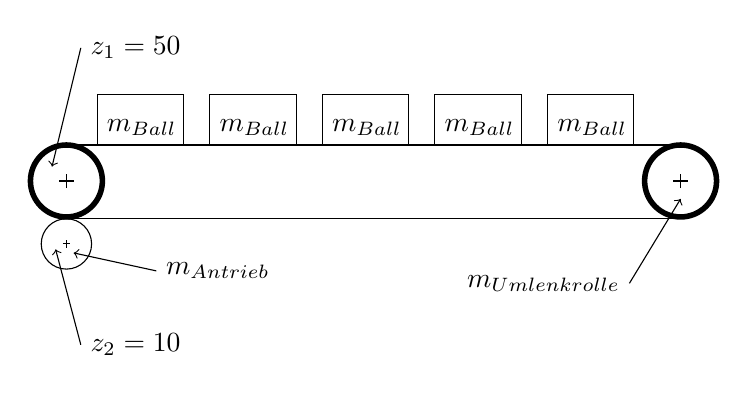
\begin{tikzpicture}[scale = 1.3]
        \draw [-,line width=2pt](0,0) circle (10pt);\draw [-,line width=2pt](6,0) circle (10pt); 
        %beide Kreise der Hauptrollen
        \draw  (0,10pt) -- (6, 10pt); \draw (0,-10.5pt) -- (6,-10.5pt); %die beiden Förderbänder-Striche
        \draw (0,-2pt) -- (0, 2pt); \draw (0cm-2pt,0) -- (0cm+2pt, 0); %Das x der ersten Rolle
        \draw (6,-2pt) -- (6, 2pt); \draw (6cm-2pt,0) -- (6cm+2pt, 0); %Das x der zweiten Rolle
        \draw [<-] (6cm-0pt , -5pt) -- (5.5,-1)node[left]{$m_{Umlenkrolle}$}; %zeige-Linie auf das 
        %Hintere Rad mit Text
        \draw (0.3,10pt)node[above right] {$m_{Ball}$} -- ++(0, 14pt)-- ++(24pt,0) -- ++(0, -14pt);
        \draw (1.4,10pt)node[above right] {$m_{Ball}$} -- ++(0, 14pt)-- ++(24pt,0) -- ++(0, -14pt);
        \draw (2.5,10pt)node[above right] {$m_{Ball}$} -- ++(0, 14pt)-- ++(24pt,0) -- ++(0, -14pt);
        \draw (3.6,10pt)node[above right] {$m_{Ball}$} -- ++(0, 14pt)-- ++(24pt,0) -- ++(0, -14pt);
        \draw (4.7,10pt)node[above right] {$m_{Ball}$} -- ++(0, 14pt)-- ++(24pt,0) -- ++(0, -14pt);
        \draw (0,-17.5pt) circle (7pt);  \draw [<-] (2pt , -20pt) -- (25pt,-25pt)node[right]
        {$m_{Antrieb}$}; %zeige-Linie auf das Antriebsrad mit Beschriftung
        \draw (-1pt,-17.5pt) -- (1pt,-17.5pt); \draw (0,-18.5pt) -- (0, -16.5pt); %Das x der zweiten Rolle
        \draw [<-] (-4pt , 4pt) -- (4pt,1.3)node[right]{$z_1 = 50$}; %zeige-Linie auf das linke 
        %Umlenkrad mit Beschriftung
        \draw [<-] (-3pt , -19pt) -- (4pt,-1.6)node[right]{$z_2 = 10$}; %zeige-Linie auf das 
        %Antriebsrad mit Beschriftung
    \end{tikzpicture}
   	\centering
    \caption{Erläuterungen zur Förderbandberechnung}
\end{figure}
\begin{align}
    M_{Motor} &= M_{Antrieb} \cdot i \label{equ:M_Antrieb}\\
    i &=\frac{z_1}{z_2}\\
    M_{Antrieb} &= F_u \cdot r_A\\
    F_u &= \mu \cdot g \cdot \left(5 \cdot m_{Ball} + m_{Umlenkrolle} + m_{Band} \right)\label{equ:F_u}
\end{align}
\\
Aus den Formeln \ref{equ:M_Antrieb} bis \ref{equ:F_u} ergibt dies benötigte Drehmoment am Motor. 
\begin{align}
    M_{Motor} &= \mu \cdot g \cdot r_A \cdot \left(5 \cdot m_{Ball} + m_{Umlenkrolle} + m_{Band}\right) 
    \cdot \frac{z_1}{z_2} \\
    n_{Motor} &=\frac{v_{Band}}{2 \cdot r_A \cdot \pi} \cdot i
\end{align}

\textbf{Berechnungswerte}\\
\begin{tabular}{lll}
	\rule{0pt}{11pt} $g$ & $9.81 \frac{N}{kg}$ & \\
	\rule{0pt}{11pt} $m_{ball}$ & $0.055 kg$ & \\
	\rule{0pt}{11pt} $m_{Umlenkrolle}$ & $0.020 kg$ & gemäss CAD \\
	\rule{0pt}{11pt} $m_{Band}$ & $0.035 kg$ & gemäss Datenblatt \\
	\rule{0pt}{11pt} $z_1$ & $50$ & gewählte Übersetzung \\
	\rule{0pt}{11pt} $z_2$ & $10$ & gewählte Übersetzung \\
	\rule{0pt}{11pt} $r_a$ & $0.020 m$ & gemäss Konstruktion \\
	\rule{0pt}{11pt} $v_{Band}$ & $0.1 \frac{m}{s}$ & vorgegebener Wert \\
\end{tabular}\\
\\
\\
\textbf{Resultate}\\
\begin{tabular}{ll}
	\rule{0pt}{11pt} $M_{motor}$ & $0.0987 Nm$ \\
	\rule{0pt}{11pt} $n_{motor}$ & $3.98 \frac{1}{s}$ \\
\end{tabular}